\documentclass[tikz,border=8pt]{standalone}
% Shared look for every TikZ diagram. Load with \input{../../tools/tikz-style.tex}
\usepackage[sfdefault]{roboto}
\usetikzlibrary{arrows.meta, positioning, shapes.geometric, calc, fit, backgrounds}
\definecolor{cblue}{HTML}{4C78A8}
\definecolor{corange}{HTML}{F58518}
\definecolor{cgreen}{HTML}{54A24B}
\definecolor{cred}{HTML}{E45756}
\definecolor{cpurple}{HTML}{B279A2}
\definecolor{cgrey}{HTML}{6B6B6B}
\tikzset{
  every picture/.style={font=\sffamily, line width=1.2pt},
  box/.style={draw=#1, fill=#1!12, rounded corners=4pt, align=center, inner sep=7pt, minimum height=1.1cm},
  box/.default=cgrey,
  arrow/.style={-{Stealth[length=3mm]}, draw=cgrey, line width=1.4pt},
  title/.style={font=\sffamily\bfseries\Large},
  note/.style={font=\sffamily\small, text=cgrey, align=center},
}
\AtBeginDocument{\hyphenpenalty=10000 \exhyphenpenalty=10000}

% Top: the robot as a MIMO system: the two wheel forces F_L, F_R each change both the speed v and the heading theta.
% V = (F_L + F_R)/(8 s + 2); Theta = (F_R - F_L)/s^2 (torque (F_R - F_L) x 0.1 m into 1/(0.1 s^2)).
% Bottom: a mixer turns the speed loop's force u and the heading loop's torque tau into wheel forces
% F_R = u/2 + 5 tau, F_L = u/2 - 5 tau, so each loop sees one input and one output (two SISO loops).
\begin{document}
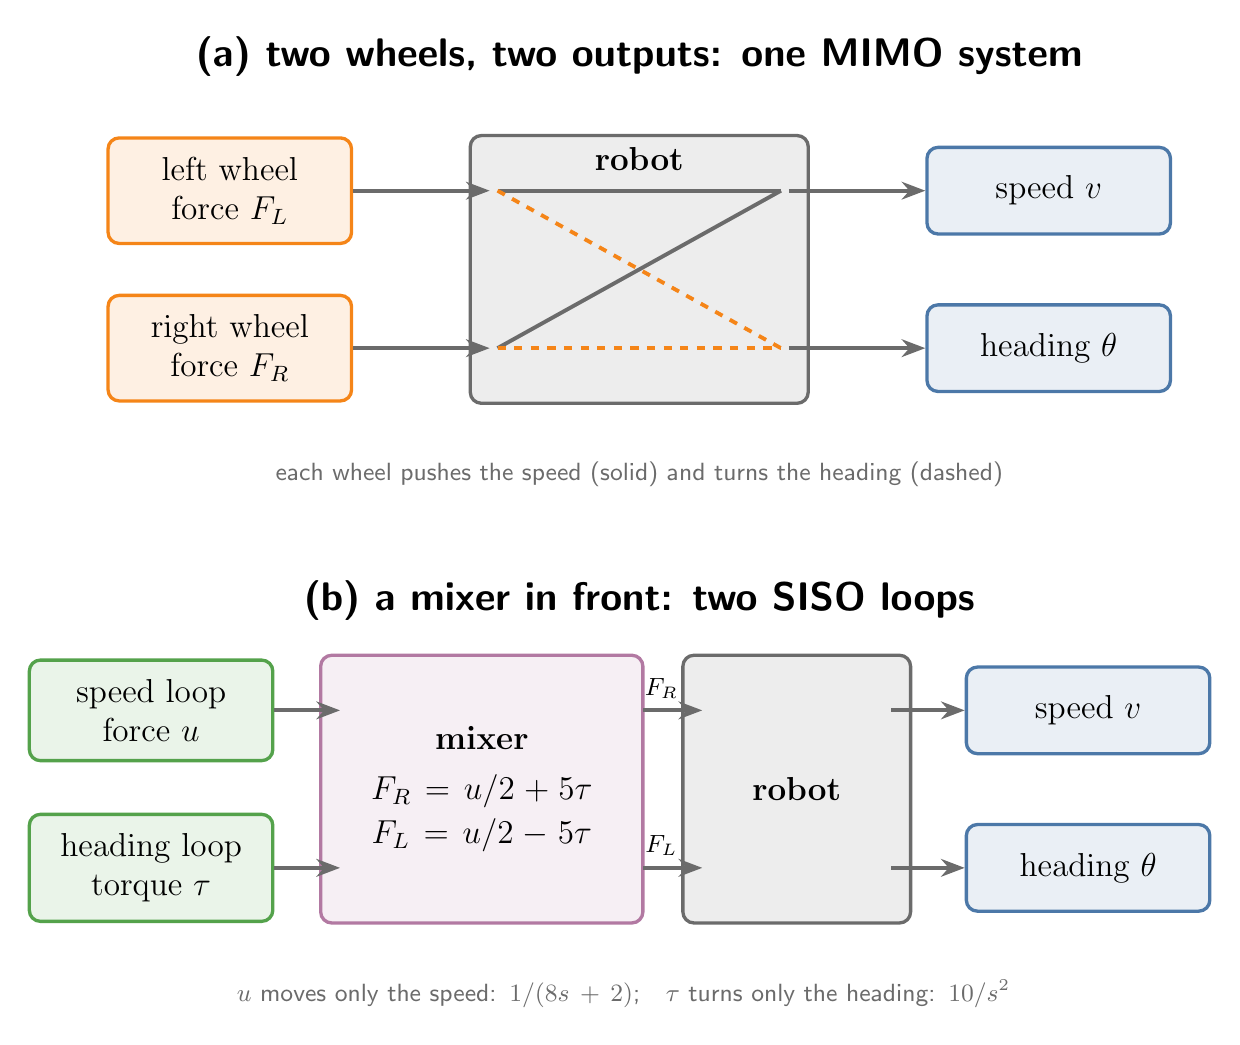
\begin{tikzpicture}[every node/.append style={font=\large}]
  % --- top: MIMO ---
  \node[title] at (5.2,3.3) {(a) two wheels, two outputs: one MIMO system};
  \node[box=corange, text width=2.6cm] (fl) at (0,1.6) {left wheel\\ force $F_L$};
  \node[box=corange, text width=2.6cm] (fr) at (0,-0.4) {right wheel\\ force $F_R$};
  \node[box=cgrey, text width=3.8cm, minimum height=3.4cm] (rob) at (5.2,0.6) {};
  \node[font=\large\bfseries] at (5.2,2.0) {robot};
  \node[box=cblue, text width=2.6cm] (v) at (10.4,1.6) {speed $v$};
  \node[box=cblue, text width=2.6cm] (th) at (10.4,-0.4) {heading $\theta$};
  \draw[arrow] (fl.east) -- (3.3,1.6);
  \draw[arrow] (fr.east) -- (3.3,-0.4);
  \draw[arrow] (7.1,1.6) -- (v.west);
  \draw[arrow] (7.1,-0.4) -- (th.west);
  \draw[cgrey, line width=1.4pt] (3.4,1.6) -- (7.0,1.6);
  \draw[cgrey, line width=1.4pt] (3.4,-0.4) -- (7.0,1.6);
  \draw[corange, line width=1.4pt, dashed] (3.4,1.6) -- (7.0,-0.4);
  \draw[corange, line width=1.4pt, dashed] (3.4,-0.4) -- (7.0,-0.4);
  \node[note, text width=11cm] at (5.2,-2.0) {each wheel pushes the speed (solid) and turns the heading (dashed)};
  % --- bottom: mixer, two SISO loops ---
  \node[title] at (5.2,-3.6) {(b) a mixer in front: two SISO loops};
  \node[box=cgreen, text width=2.6cm] (u) at (-1.0,-5.0) {speed loop\\ force $u$};
  \node[box=cgreen, text width=2.6cm] (tau) at (-1.0,-7.0) {heading loop\\ torque $\tau$};
  \node[box=cpurple, text width=3.6cm, minimum height=3.4cm] (mix) at (3.2,-6.0) {\textbf{mixer}\\[4pt] $F_R = u/2 + 5\tau$\\[2pt] $F_L = u/2 - 5\tau$};
  \node[box=cgrey, text width=2.4cm, minimum height=3.4cm] (rob2) at (7.2,-6.0) {\textbf{robot}};
  \node[box=cblue, text width=2.6cm] (v2) at (10.9,-5.0) {speed $v$};
  \node[box=cblue, text width=2.6cm] (th2) at (10.9,-7.0) {heading $\theta$};
  \draw[arrow] (u.east) -- (1.4,-5.0);
  \draw[arrow] (tau.east) -- (1.4,-7.0);
  \draw[arrow] (5.25,-5.0) -- (6.0,-5.0);
  \draw[arrow] (5.25,-7.0) -- (6.0,-7.0);
  \node[font=\small] at (5.48,-4.72) {$F_R$};
  \node[font=\small] at (5.48,-6.72) {$F_L$};
  \draw[arrow] (8.4,-5.0) -- (v2.west);
  \draw[arrow] (8.4,-7.0) -- (th2.west);
  \node[note, text width=12cm] at (5.0,-8.6) {$u$ moves only the speed: $1/(8s + 2)$;\quad $\tau$ turns only the heading: $10/s^2$};
\end{tikzpicture}
\end{document}
